\section{Spectroscopic ETC}
\label{sec:spectroscopy}

Spectroscopy divides the same photons that photometry collects into
hundreds or thousands of wavelength bins, so its S/N per bin is lower by
$\sqrt{N_{\rm bins}}$-like factors and every loss mechanism bites harder.
Two geometries are modelled, and they fail in opposite ways. A
\emph{slit} spectrograph defines its resolution optically and pays for it
at the entrance: slit losses, extraction losses, and --- unless the slit
tracks the parallactic angle --- chromatic losses from atmospheric
dispersion that can silently remove half the blue signal. A
\emph{slitless} grating (the Star Analyser class) pays nothing at an
entrance it does not have, collects every photon of source \emph{and}
sky at every wavelength, and instead surrenders resolution to the
seeing: its resolution element is the star image itself, dispersed. The
engine treats both with the same per-element bookkeeping so that their
trade-off can be compared honestly for the same hardware.

All spectroscopic quantities are per resolution element (``resel''): the
wavelength interval $\Delta\lambda$ the instrument cannot subdivide, one
output row of the ETC. The wavelength grid
is logarithmic at constant $R$ in slit mode, or linear with the resolution
element $\Delta\lambda = \mathcal{D}\,\ell$ in slitless mode
($\mathcal{D}$ = dispersion in \si{\angstrom}/pixel, $\ell$ = LSF FWHM in
pixels). Source and sky rates follow Eq.~(\ref{eq:rate}) restricted to each
element, and the S/N applies Eq.~(\ref{eq:snr}) with
$N_{\rm pix}$ = (dispersion pixels per element) $\times$ (spatial extraction
pixels).

\subsection{Per-element integration: why bin integrals, not samples}
\label{sec:binint}

How the template flux is booked into resolution elements decides whether
line spectroscopy is trustworthy. Sampling the template at the element's
central wavelength and multiplying by $\Delta\lambda$ — the obvious
shortcut — is correct only for spectra smooth on the scale of
$\Delta\lambda$. For a spectral \emph{line} narrower than the element it
is wrong in a way that depends on luck: the line is fully counted if a
sample lands on it and lost if none does, so the \emph{total} detected
line flux changes with the chosen $R$ — unphysical, since dispersing the
same photons more or less finely cannot create or destroy them. The
v10.1 audit measured an $8\times$ spread in the detected counts of a
\SI{2}{\angstrom} emission line between $R = 200$ and $R = 20000$ under
point sampling. Since v10.2 each element's source counts are the exact
\emph{integral} of the calibrated template over the element,
\begin{equation}
  \dot S_i \;=\; \eta\,A \int_{\lambda_i - \Delta\lambda_i/2}
  ^{\lambda_i + \Delta\lambda_i/2}
  \flam^{\rm cal}\, T_\lambda\, Q_\lambda\, O_\lambda\,
  T_{\rm atm}^{\,X}\, \frac{\lambda}{hc}\, d\lambda ,
\end{equation}
evaluated for all elements at once by cumulative trapezoidal integration
on the union of the template grid and the element edges (exact for the
piecewise-linear tabulated inputs, and $O(n)$ — a single pass even at
$R = 10^5$). Total line counts are now invariant under $R$ to better
than 0.2\% (regression-tested), and $\sigma(\mathrm{EW})$
(Sect.~\ref{sec:ew}) inherits that reliability.

\subsection{Slit mode}
\label{sec:slit}

The extracted fraction is the product of two couplings of
Eq.~(\ref{eq:slit}): the slit width across dispersion and the finite
extraction height along it. When the slit is \emph{not} at the parallactic
angle of Eq.~(\ref{eq:parallactic}), the differential refraction
$\Delta R(\lambda)$ of Eq.~(\ref{eq:dr}) decentres the PSF in the slit per
wavelength; \spetc{} applies the worst-case geometry (full offset
perpendicular to the slit), reproducing the classical
\citet{filippenko1982} blue-end losses (Fig.~\ref{fig:dispersion}). A
measured slit-width/resolving-power curve, when supplied, overrides the
nominal $R$.

\subsection{Slitless mode and the Star Analyser}
\label{sec:slitless}

In slitless spectroscopy the resolution element is set by the image quality,
not by a slit: $\ell = \sqrt{(s/p)^2 + \ell_0^2 + \ell_{\rm AD}^2}$ combines
seeing, the intrinsic grating LSF and the atmospheric-dispersion smear
within one element ($s$ = seeing FWHM, $p$ = plate scale, $\ell_0$ =
intrinsic LSF in pixels, $\ell_{\rm AD}$ = dispersion smear in pixels).
The sole extraction aperture is the cross-dispersion height.

\paragraph{The slitless sky is a full-bandpass background.} The decisive
physical difference from a slit is what happens to the \emph{sky}.
Dispersing a spatially \emph{uniform} source leaves the detector
illumination uniform: every wavelength of sky lands on every pixel,
merely shifted, and the shifts of a uniform field are invisible. A
slitless pixel therefore receives the sky integrated over the
\emph{entire} grating bandpass,
\begin{equation}
  \dot B_{\rm pix} \;=\; p^2\, \eta\, A\, \varepsilon_g
  \int_{\lambda_{\rm min}}^{\lambda_{\rm max}}
  \mu_\lambda^{\rm sky}\, T_\lambda\, Q_\lambda\, O_\lambda\,
  \frac{\lambda}{hc}\, d\lambda ,
  \label{eq:slitless-sky}
\end{equation}
with $\mu_\lambda^{\rm sky}$ the sky spectral surface brightness per
arcsec$^2$, $p^2$ the pixel solid angle and $\varepsilon_g$ the grating
efficiency; the sky per element is $\dot B_{\rm pix}$ times the
extraction pixels. This is the classical reason objective-grating spectra
are sky-limited. Booking only one element's $\Delta\lambda$ of sky per
pixel — as a slit would allow — underestimates the background by the
ratio (bandpass width)/(element width), about two orders of magnitude for
a Star Analyser covering \SI{3300}{\angstrom} with \SI{28}{\angstrom}
elements; the v10.1 audit measured a $118\times$ deficit, corrected in
v10.2 and regression-tested. Practical consequence: slitless S/N under a
bright sky is far worse than a slit ETC intuition suggests, and the
mode's advantage survives only for short exposures on brighter targets —
which is precisely how Star Analysers are productively used.

For a transmission grating in the converging beam --- the Star Analyser
100/200 geometry --- the first-order deviation is
$x \simeq L\,m\,n\,\lambda$, so the dispersion at the detector is
\begin{equation}
  \mathcal{D} \;=\; \frac{10^{4}\, p_{\mu m}}{L_{\rm mm}\; n_{\rm mm}\; m}
  \quad [\si{\angstrom}/\text{pixel}],
  \label{eq:sa}
\end{equation}
with $n$ the groove density (100 or 200 mm$^{-1}$), $L$ the
grating-to-sensor distance and $m=1$. An SA100 at $L=\SI{42}{mm}$ on
\SI{4.63}{\micro\metre} pixels gives $\mathcal{D} = 11.0$
\si{\angstrom}/pixel, matching its published calibration; an SA200 at the
same distance gives half that. An optional scalar first-order grating
efficiency multiplies source and sky alike. Under $2.5''$ seeing the
effective resolving power is $R \simeq 100$--200
(Fig.~\ref{fig:sa100}), which is why the mode remains flagged
\emph{experimental} until validated against a calibrated instrument.

\begin{figure}
  \centering
  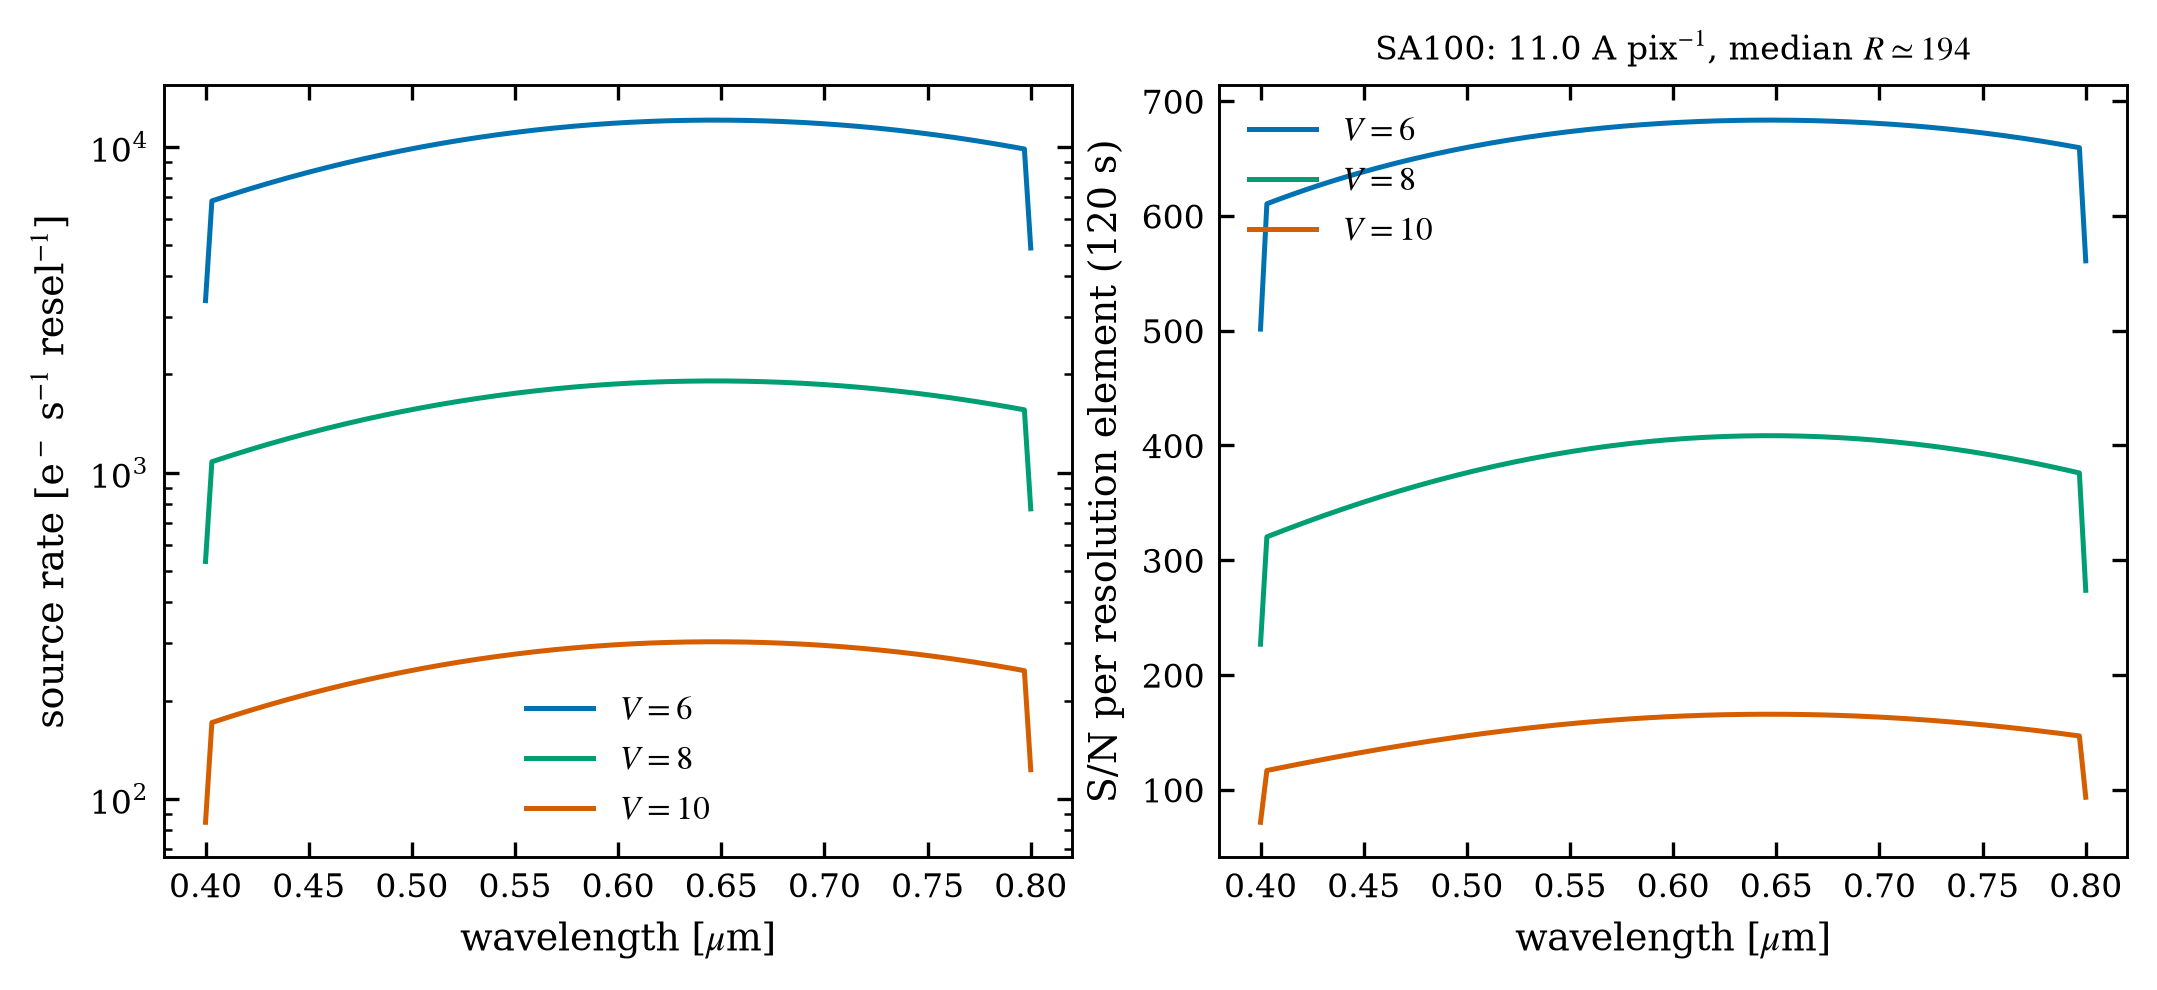
\includegraphics[width=\textwidth]{figures/fig_07_sa100.png}
  \caption{Star Analyser 100 predictions from the released code for a
  200-mm f/5 telescope with a typical CMOS camera: detected source rate
  (left) and S/N per resolution element in \SI{120}{s} (right) for
  $V = 6, 8, 10$ flat-spectrum targets.}
  \label{fig:sa100}
\end{figure}

\subsection{Slit-spectrograph geometry}
\label{sec:geometry}

Amateurs know their spectrograph by its hardware — groove density $n$,
collimator and camera focal lengths $f_{\rm coll}, f_{\rm cam}$, slit
width — not by $R$. In the Littrow approximation the grating equation
gives $\sin\beta = m n \lambda/2$ and a reciprocal linear dispersion
$d\lambda/dx = \cos\beta \cdot 10^{7}/(m\,n\,f_{\rm cam})$
[\si{\angstrom}/mm]. The resolution element on the detector is the
narrower of the geometric slit image and the seeing image, both reimaged
by $f_{\rm cam}/f_{\rm coll}$ (anamorphism 1 in Littrow):
\begin{equation}
  \Delta\lambda = \min(w_{\rm slit}, w_{\rm seeing})\,
  \frac{f_{\rm cam}}{f_{\rm coll}}\,\frac{d\lambda}{dx},
  \qquad R = \frac{\lambda}{\Delta\lambda},
\end{equation}
with the widths converted from arcsec at the telescope focal plane. The
calculator reports whether the configuration is slit- or seeing-limited
and feeds the ETC's resolving-power field, which remains editable; an
LHIRES III-like configuration (2400 lines/mm, $f=200$~mm Littrow, 25-\si{\micro\metre}
slit) returns $R \simeq 2\times10^4$ at H$\alpha$, in line with the
instrument's specification.

Two guards keep the entered $R$ honest (v10.2). With the geometry
supplied and the clamp option enabled, the engine itself limits the
entered $R$ to the geometry's value at the band centre — a physically
impossible $R$ can then no longer silently inflate every per-element
prediction. Conversely, when the seeing disc is much \emph{narrower}
than the slit the delivered resolution is set by the star image, i.e.\
finer than the slit-limited $R$; the engine flags this case so the user
knows the reported $R$ is conservative.

\subsection{Equivalent-width detectability}
\label{sec:ew}

The spectroscopic S/N is turned into a science answer through the
\citet{cayrel1988} relation for the equivalent-width uncertainty of a line
of FWHM $W$ sampled with pixels of width $\delta x$:
\begin{equation}
  \sigma(\mathrm{EW}) \;\simeq\; \frac{1.5\,\sqrt{W\,\delta x}}
  {(\mathrm{S/N})_{\rm pixel}},
  \label{eq:cayrel}
\end{equation}
evaluated per wavelength with the resolution element as $W$ and reported
in m\AA{} in every result table. The practical criterion: a line is
securely measurable when its expected equivalent width exceeds
$\simeq 3\,\sigma(\mathrm{EW})$ — e.g.\ $\sigma(\mathrm{EW}) = 15$~m\AA{}
means H$\alpha$ variations of a Be star at the 50~m\AA{} level are
detectable, while 20~m\AA{} photospheric lines are marginal.

\subsection{Time series and reverse solving}

Planning series evaluate the S/N reference wavelength bin at every time
sample of the visibility window (full spectra only at the selected time and
the plot-slider samples), with the sky model, airmass, refraction and
parallactic angle recomputed per sample. Target-S/N requests use the
closed-form solver of Sect.~\ref{sec:noise} per element and are checked
against the saturation limit rather than being silently declared feasible.
